Die Messdaten müssen sicher, einfach zugänglich und möglichst Speichereffizent abgelegt werden.
Dafür eigent sich InfluxDB\footnote{influxdata.com} in kombination mit einem Grafana\footnote{Grafana.com} Webinterface
\subsection{InfluxDB}
InfluxDB ist eine von InfluxData entwikelte Open Source Time Series Database. 
Time Series Database  sind darauf optimeirt zusammengehörige Paare von Zeit(en) und Wert(en) zu verwalten und zu Komprimieren.
InfluxDB hat eine große Benutzer- und Entwicklerbasis, es gibt vielseitige Interfaces um Daten zu visualisieren, darunter Grafana.
Eine Time Series Database eignet sich für den Messaufbau da die Spectralmessdaten mit Zeitbezug erfasst werden.

\subsection{Grafana}
Grafana ist eine Open Source Anwendung zur grafischen Darstellung von Daten aus verscheidenden Datenbanken(InfluxDB,  MySQL,...) in einem Webinterface.
Das Webinterface ermöglicht sogenannte Dashboards (Abb. \ref{fig:Beispiel_Grafana_Dashboard}) anzulegen, in welchen die gespeicherten Daten vielseitig dargestellt werden können.
Außerdem können die Daten im CSV-Format exportiert werden.
Die Webschnittstelle eignet sich für den Messaufbau, da sie eine leicht verständliche Live-Überwachung der Messungen bietet.
\begin{figure}[ht!]
\centering
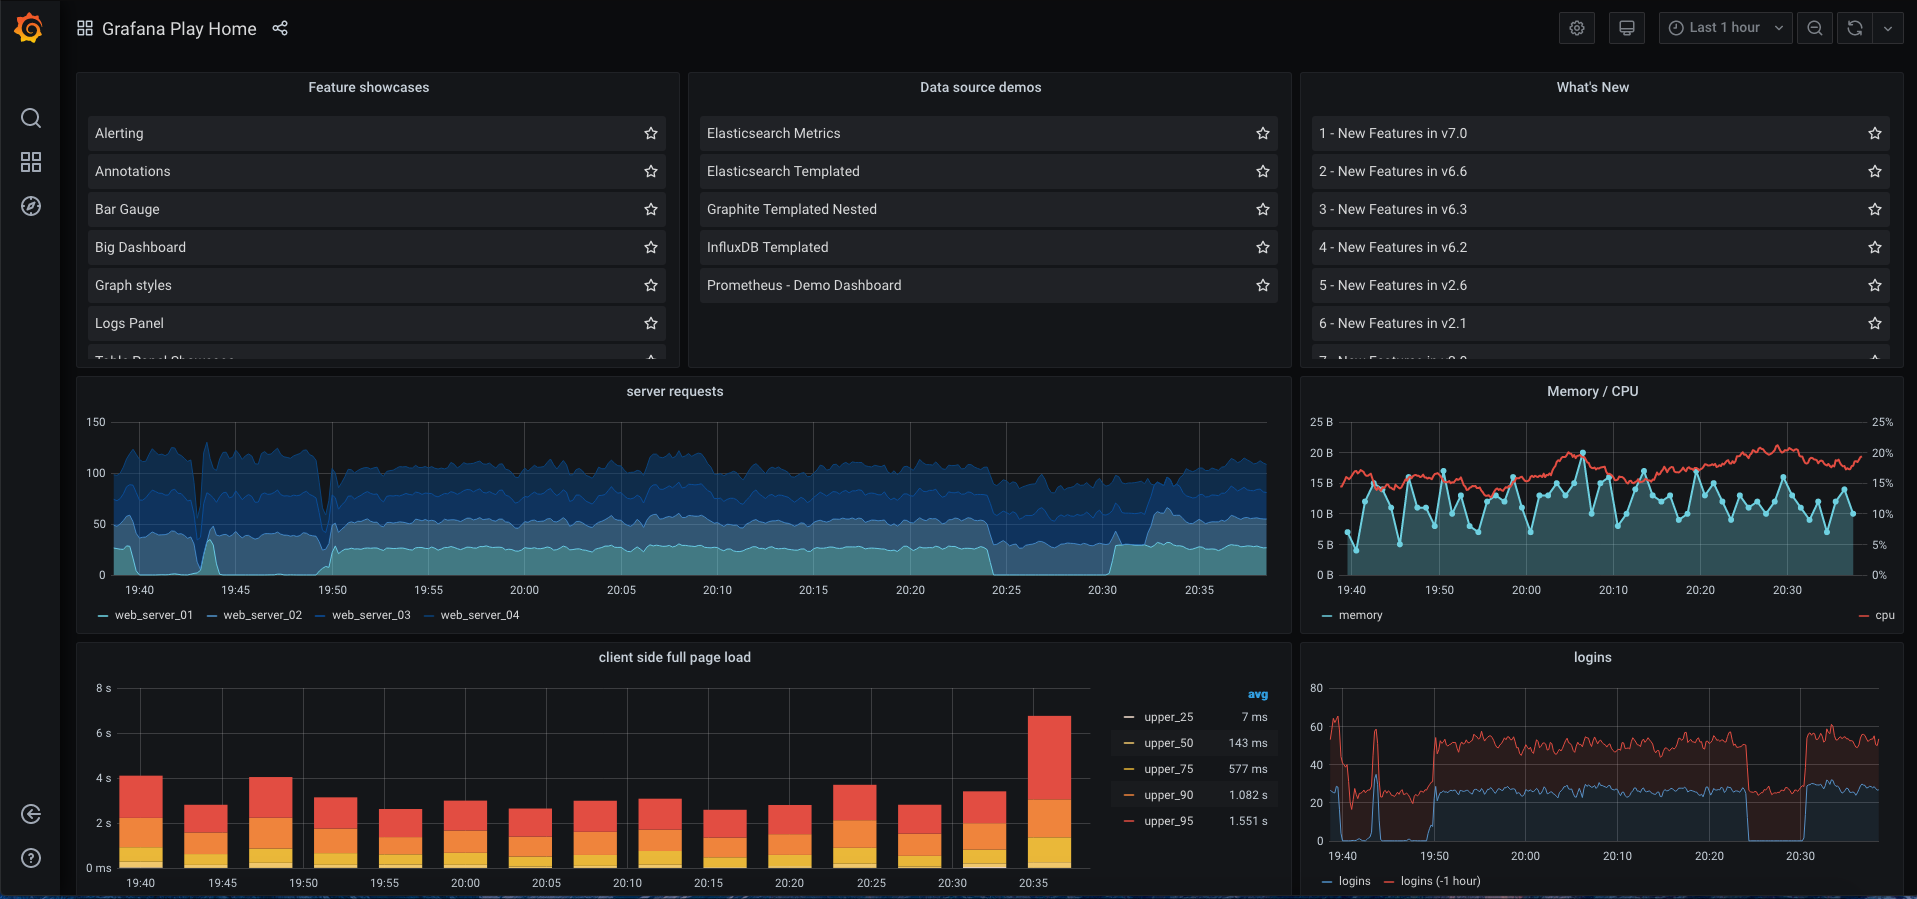
\includegraphics[width=0.75\textwidth]{img/Beispiel_Grafana_Dashboard}
\caption{Beispiel Grafana Dashboard}
\label{fig:Beispiel_Grafana_Dashboard}
\end{figure}